% =====================================================================
% TwinCheck -- MAAI902 (NLP & LLMs) group report. DRAFT v1 (23 Nov 2026).
% Lead: Himasri. Compile with pdflatex + bibtex (Overleaf default).
% Files: main.tex, refs.bib, figures/fig_entail_shortcut.png
% Every number comes from a file in results/ (path given in comments).
% =====================================================================
\documentclass[11pt,a4paper]{article}

\usepackage[margin=2.4cm]{geometry}
\usepackage[T1]{fontenc}
\usepackage{lmodern}
\usepackage{microtype}
\usepackage{booktabs}
\usepackage{tabularx}
\usepackage{graphicx}
\usepackage{amsmath,amssymb}
\usepackage{xcolor}
\usepackage{caption}
\usepackage[numbers,sort&compress]{natbib}
\usepackage[hidelinks]{hyperref}
\Urlmuskip=0mu plus 2mu
\renewcommand{\UrlBreaks}{\do\/\do\-\do\_\do\.}

\captionsetup{font=small,labelfont=bf}
\setlength{\parskip}{0.35em}
\newcommand{\tw}[1]{\texttt{\_#1}}          % twin suffix, e.g. \tw{B}
\newcommand{\pp}{\,pp}                      % percentage points
\newcommand{\stagebox}[2]{\fbox{\parbox[c][1.25cm][c]{2.45cm}{\centering\small\textbf{#1}\\[2pt]\footnotesize #2}}}

\title{\textbf{TwinCheck: Do Bilingual Fact-Checking Models Follow the Evidence?}\\[4pt]
\large Testing and training with one-change ``twins'' in English, Arabic and mixed text\\[2pt]
\normalsize MAAI902 Natural Language Processing and Large Language Models}
\author{%
\begin{tabular}{c@{\hspace{3em}}c}
Himasri & Rathi \\
\small University of Wollongong in Dubai & \small University of Wollongong in Dubai \\[10pt]
Youssef & Feba \\
\small University of Wollongong in Dubai & \small University of Wollongong in Dubai
\end{tabular}}
\date{November 2026}

\begin{document}
\maketitle

\begin{abstract}
\noindent
Automated fact-checkers reach respectable scores on public benchmarks, yet several studies show that they can do so without reading the evidence they are given. We present TwinCheck, a bilingual English--Arabic fact-checking pipeline that extracts claims from a message, retrieves and ranks evidence, scores each snippet with natural language inference (NLI), and returns a calibrated verdict (supported, contradicted or unverified) with a cited explanation. To test whether a verdict changes for the right reason, we build \emph{twins}: copies of real claims that change exactly one thing, such as rewording the claim, translating it, swapping one entity in the evidence, or replacing the evidence with unrelated text. We use twins both to audit models and to train a small verdict head with a \emph{twin loss}. On MultiFC, the twin loss raises the share of swapped-evidence twins called contradicted from 52\% to 90\% and of unrelated-evidence twins called unverified from 42\% to 100\%, for a loss of about one macro-F1 point. The most accurate systems in our study, a claim-only classifier and a fine-tuned Qwen3-4B, fail these tests, which shows that accuracy alone can favour models that ignore the evidence.
\end{abstract}

% ---------------------------------------------------------------------
\section{Rationale, Problem Statement and Objectives}
% ---------------------------------------------------------------------

\paragraph{Rationale.}
Forwarded messages are a common route for rumours in the UAE. They often mix Arabic and English and bundle several claims into one text. Professional fact-checkers publish careful verdicts, but one claim at a time and usually after the message has spread. Automated fact-checking can help at scale only if people can see \emph{why} a verdict was reached: the verdict should rest on evidence, cite it, and not change when the same claim is written in another language.

\paragraph{Problem statement.}
Evidence-based fact-checking is usually framed as: given a claim and retrieved evidence, predict a verdict \citep{thorne2018fever,augenstein2019multifc}. Prior work has shown that strong benchmark scores do not guarantee that the evidence is used. On MultiFC, \citet{hansen2021reason} found that models scored as well from the evidence alone as from claim and evidence together, and concluded that they were not reasoning over the pair. \citet{glockner2022missing} found that for 70\% of MultiFC's false claims at least one saved search snippet came from a fact-checking article that already stated the verdict; a BERT model scored 59.7 macro-F1 on PolitiFact claims with such leaked snippets and 25.6 without them. On the cleaner AVeriTeC benchmark \citep{schlichtkrull2023averitec}, the 2024 shared-task winner reported that GPT-4o reached 71.0\% accuracy with no evidence against 72.4\% with its full pipeline \citep{rothermel2024infact}. In multimodal checking, \citet{papadopoulos2025similarity} showed that claim--evidence \emph{similarity} can pass for factuality. We extend that observation to text.

Two lines of work test evidence use more directly. VitaminC \citep{schuster2021vitaminc} built pairs in which a small edit to a Wikipedia sentence flips the answer, and CCN \citep{abdelnabi2022ccn} compared models with and without real web evidence. These studies motivate our design, but the first uses clean English Wikipedia, and the second measures evidence use on average rather than for each claim. In Arabic, X-FACT \citep{gupta2021xfact} found that a claim-only model nearly matched evidence-based ones, and to our knowledge no X-FACT or M4FC study checks whether the same claim receives the same verdict across languages.

\paragraph{Objectives and research questions.}
We ask whether a verdict changes when, and only when, the evidence changes:
\begin{itemize}\setlength{\itemsep}{1pt}
  \item \textbf{RQ1:} Do current approaches change their verdict when the evidence changes, and keep it when only wording or language changes?
  \item \textbf{RQ2:} Can training with twins make a model follow the evidence at little cost in accuracy?
  \item \textbf{RQ3:} Does this hold for Arabic and mixed Arabic--English claims?
\end{itemize}
Our target was to raise the twin metrics while losing at most one point of macro-F1. To our knowledge, our contributions are: (i) one-change twins built from real fact-checked claims with web evidence, covering evidence swaps, unrelated evidence, paraphrases, Arabic and mixed text; (ii) a twin loss that trains a verdict head to follow the evidence; (iii) an English, Arabic and mixed evaluation of cross-lingual consistency; and (iv) evidence that accuracy and evidence-reading diverge on MultiFC.

% ---------------------------------------------------------------------
\section{Dataset Description and Pre-processing}
% ---------------------------------------------------------------------

\subsection{Datasets}
We use four public datasets (Table~\ref{tab:data}). MultiFC \citep{augenstein2019multifc} collects real claims from 26 fact-checking websites, each with up to ten Google search snippets saved at collection time. Its official test labels were never released, so we use only the labelled train and validation files and make our own split. AVeriTeC \citep{schlichtkrull2023averitec} provides question--answer evidence written by annotators from web pages published before each claim; we turn each answer into one ``question? answer'' snippet and use it as a clean second English test. X-FACT \citep{gupta2021xfact} supplies Arabic claims, all from misbar.com, with search snippets. M4FC \citep{geng2025m4fc} provides real Arabic claims without evidence text; following its authors' advice, we use it for evaluation only.

\begin{table}[t]
\centering\small
\caption{Datasets used. Counts are after label mapping and cleaning (\texttt{results/R1}, \texttt{notes/Y1.md}).}
\label{tab:data}
\begin{tabularx}{\textwidth}{@{}l X X@{}}
\toprule
Dataset (role) & Key facts & Caveat $\rightarrow$ our response \\
\midrule
MultiFC (main English train/val/test) & 21,057 claims kept: 16,847 / 2,104 / 2,106; up to 10 Google snippets each & Hidden test labels $\rightarrow$ own split; leaked snippets $\rightarrow$ removed \\
AVeriTeC (clean English test) & 2,990 claims (2,309 / 252 / 429); human Q\&A evidence from pages dated before the claim & ``Conflicting'' label $\rightarrow$ dropped (233 claims) \\
X-FACT Arabic (Arabic NLI data, test) & 2,090 Arabic claims; 919 kept after mapping; 135 test claims & 91\% false $\rightarrow$ macro-F1, balanced twins; misbar.com snippets removed \\
M4FC Arabic (real Arabic test) & 614 Arabic claims (613 false) plus 156 true captions; no evidence text & Evaluation-only use, as its authors advise \\
\bottomrule
\end{tabularx}
\end{table}

\subsection{Label mapping and cleaning}
Each fact-checking site uses its own rating words, such as ``pants on fire!'', ``fiction!'' or ``4 Pinocchios''. We listed all 116 MultiFC labels that occur in the train and validation files and mapped each by hand to \emph{supported}, \emph{contradicted} or \emph{unverified} (\texttt{data/label\_map.csv}). Labels that are not clearly about truth (half true, mixture, misleading, satire, and PolitiFact promise ratings) were dropped, following \citet{hansen2021reason}; this removed 9,877 of 31,433 MultiFC claims. When a label's meaning was unclear, we dropped it rather than guess.

Cleaning (\texttt{src/data/clean.py}) applies the same rules to every dataset. First, it removes snippets from fact-checking websites, the leak described by \citet{glockner2022missing}: 25,993 MultiFC snippets, including 13,585 from politifact.com and 4,002 from snopes.com. Second, it removes snippets that overlap the claim by more than 90\%, since they repeat the claim rather than test it (16,769 snippets). Third, it removes duplicate claims and keeps at most ten snippets per claim. Claims left without snippets (426) are set aside. MultiFC shrinks from 197,258 to 154,277 snippets. We split it 80/10/10, stratified by label, with seed 42. The classes are imbalanced (34\% supported, 63\% contradicted, 3.5\% unverified), so all main results use macro-F1, which weights each class equally.

\subsection{Augmentation: twins}
Twins are our main form of data augmentation (Table~\ref{tab:twins}). Sources are supported claims with at least two relevant snippets, fixed with seed 42: 500 test and 3,000 training sources. A paraphrase twin (\tw{P}) rewords the claim with Qwen3-8B and is kept only if spaCy finds the same names, dates and numbers. An evidence-swap twin (\tw{B}) replaces one place, person or date in every snippet that mentions it, using values from our own data, so the correct verdict becomes contradicted. An unrelated twin (\tw{C}) replaces the evidence with snippets from a claim that shares no entities and has reranker relevance below 0.1, so the correct verdict becomes unverified. For 200 test sources, Arabic twins translate the claim and evidence (\tw{A}), or only the claim (\tw{M}), with Qwen3-8B and a 3,044-name glossary; swaps are made in English before translation. Twins always keep the split of their source.

\begin{table}[t]
\centering\small
\caption{Twin types and counts (\texttt{results/R3}, \texttt{results/Y4}).}
\label{tab:twins}
\begin{tabular}{@{}llll@{}}
\toprule
Twin & What changes & Correct verdict & Test count \\
\midrule
\tw{P} paraphrase & claim reworded, same entities & same as original & 174 \\
\tw{A} Arabic & claim and evidence in Arabic & same as original & 147 \\
\tw{M} mixed & Arabic claim, English evidence & same as original & 192 \\
\tw{B} evidence swap & one entity swapped in the evidence & contradicted & 281 (+145 Arabic) \\
\tw{C} unrelated & evidence from an unrelated claim & unverified & 500 (+158 Arabic) \\
\midrule
\multicolumn{3}{@{}l}{English training twins (from 3,000 sources)} & 5,705 \\
\bottomrule
\end{tabular}
\end{table}

\paragraph{Quality checks and gold sets.}
Two team members checked 120 test twins by hand, 30 of them jointly (Cohen's $\kappa=0.57$ \citep{cohen1960kappa}, 83\% raw agreement). Almost all \tw{P} (97.5\%) and \tw{C} (100\%) twins were valid, but only 22.5\% of \tw{B} twins were clean contradictions of the claim; common faults were nonsense entities, surname-only swaps and swaps that did not touch the claim (\texttt{results/H4/handcheck\_summary.json}). Of 50 checked translations, 27 (54\%) were fully correct. We also built two hand-labelled gold sets, used for testing only: 300 snippet--claim NLI pairs (150 English, 150 Arabic) and 300 WhatsApp-style messages with gold claims (102 English, 99 Arabic, 99 mixed).

% ---------------------------------------------------------------------
\section{Solution Architecture}
% ---------------------------------------------------------------------

Figure~\ref{fig:pipeline} shows the pipeline (\texttt{src/pipeline.py}). The demo receives only a message. It retrieves evidence from an offline library and generates a cited explanation, which makes it a retrieval-augmented generation (RAG) system \citep{lewis2020rag}. In the experiments, each dataset claim already carries its own snippets, so retrieval is skipped and the attached snippets go straight to the reranker. This keeps the evidence under our control, which the twin tests require, and isolates the verdict from search quality; retrieval is evaluated separately.

\begin{figure}[t]
\centering
\stagebox{1 Claims}{Qwen3-8B, 4-bit} $\rightarrow$
\stagebox{2 Retrieval}{BM25 + BGE-M3} $\rightarrow$
\stagebox{3 Reranker}{bge-reranker-v2-m3} $\rightarrow$
\stagebox{4 NLI}{mDeBERTa-v3} \\[6pt]
$\rightarrow$ \stagebox{5 Verdict head}{MLP + twin loss} $\rightarrow$
\stagebox{6 Calibration}{temperature + $\tau$} $\rightarrow$
\stagebox{7 Explanation}{Qwen3-8B, cites [1]--[3]}
\caption{TwinCheck pipeline. Steps 2--3 (retrieval) and 7 (generation) form the RAG part used in the demo; experiments feed each claim's attached snippets directly to step 3. spaCy entities feed the verdict head.}
\label{fig:pipeline}
\end{figure}

\paragraph{Claim extraction.} Qwen3-8B \citep{qwen2025qwen3}, loaded in 4-bit, receives six examples (two per language) and returns a JSON list of checkable claims in the message's language. We chose an open model so that messages never leave our own GPU, and because Qwen3 was trained on 119 languages including Arabic.

\paragraph{Evidence retrieval.} For the demo, all 163,244 cleaned snippets (MultiFC, AVeriTeC, X-FACT Arabic) are indexed twice: with BM25 for keyword matching \citep{robertson2009bm25}, and with BGE-M3 \citep{chen2024bgem3} dense embeddings in a FAISS index for meaning-based matching across languages \citep{johnson2019faiss}. The top 20 results of each are merged.

\paragraph{Relevance.} A cross-encoder reranker (\texttt{BAAI/bge-reranker-v2-m3}) reads the claim and each snippet together and returns a relevance score; in the demo it keeps the best five. The bi-encoder is fast because snippets are embedded in advance, while the cross-encoder is slower but more careful.

\paragraph{Natural language inference.} An NLI model labels each (snippet, claim) pair as entailment, contradiction or neutral. We use \texttt{mDeBERTa-v3-base-xnli-multilingual-nli-2mil7} \citep{laurer2022mdeberta,he2023debertav3} zero-shot, that is, as released after training on MNLI- and XNLI-style data \citep{conneau2018xnli}.

\paragraph{Verdict head.} For each claim, ten features summarise the evidence: relevance-weighted entailment, contradiction and neutral probability; the strongest entailment and contradiction among relevant snippets; the share of relevant snippets; entity match for place, date and person, the share of the claim's spaCy entities \citep{honnibal2020spacy} found in the evidence text (string matching, so English only); and the number of snippets. A multilayer perceptron (10 $\rightarrow$ 64 $\rightarrow$ 3, dropout 0.2, about 900 weights) maps them to three verdict probabilities. By design the verdict head never sees the image-authenticity score from the vision side of the project, so an AI-looking photo cannot by itself turn a true post into ``fake''.

\paragraph{Calibration and explanation.} Temperature scaling \citep{guo2017calibration} and an ``unverified'' threshold $\tau$ are fitted on validation data. Qwen3-8B then writes one or two sentences in the claim's language, citing only the top three snippets as [1]--[3].

\paragraph{How each model was chosen.} Every component was compared with at least one alternative on our own data (Table~\ref{tab:choices}). Where a larger model was not clearly better, we kept the smaller one.

\begin{table}[t]
\centering\small
\caption{Model selection (\texttt{results/Y3}, \texttt{R5}, \texttt{R2}, \texttt{H5}, \texttt{H7}).}
\label{tab:choices}
\begin{tabularx}{\textwidth}{@{}l l X X@{}}
\toprule
Step & Chosen & Compared with & Evidence \\
\midrule
Claims & Qwen3-8B, 4-bit, few-shot & rule-based splitter; Qwen3-4B & F1 0.984 vs 0.786; 4B 0.977 \\
Retrieval & BM25 + BGE-M3 hybrid & each alone & recall@5 EN 0.945 vs 0.91 / 0.87; AR 0.92 vs 0.86 / 0.80 \\
Relevance & reranker, fine-tuned & off the shelf; removed & accuracy 0.719 $\rightarrow$ 0.980; removal costs 5 F1, 21 ESR points \\
NLI & mDeBERTa-v3-base & XLM-R-large; DeBERTa-v3-large; two fine-tuned versions & confidence intervals overlap; one model for EN and AR; fastest \\
Verdict & MLP + twin loss & logistic regression; LightGBM & +8.5 to +9.3 ESR over twins-as-data ($p<0.001$) \\
Explanation & Qwen3-8B & Qwen3-4B & faithfulness 0.320 vs 0.352 \\
\bottomrule
\end{tabularx}
\end{table}

% ---------------------------------------------------------------------
\section{Model Training and Fine-Tuning}
% ---------------------------------------------------------------------

\subsection{Twin loss}
Standard training rewards only the right answer on original claims. The twin loss adds two terms that reward the right \emph{reason}:
\begin{equation}
\mathcal{L} = \mathrm{CE}_w(\text{orig}) + \lambda_{\text{inv}}\,\mathrm{KL}\big(p_{\text{orig}} \,\|\, p_{\text{twin}}\big)_{\{P,A,M\}} + \lambda_{\text{sens}}\,\mathrm{CE}\big(\text{\tw{B}}\!\rightarrow\!\text{contradicted},\ \text{\tw{C}}\!\rightarrow\!\text{unverified}\big).
\end{equation}
The first term is class-weighted cross-entropy on originals. The second asks paraphrase, Arabic and mixed twins to keep the original's probabilities; the original's distribution is detached so that only the twin moves. The third pushes swapped-evidence twins to contradicted and unrelated-evidence twins to unverified. Each batch holds 64 originals together with their twins. Because the KL term needs gradients, tree models cannot use this loss, which is why the head is a small neural network.

\subsection{Training settings and selection}
The head is trained with Adam (learning rate $10^{-3}$) for at most 30 epochs, with early stopping on validation macro-F1 (patience 5). We searched $\lambda_{\text{inv}} \in \{0, 0.5, 1, 2\}$ and $\lambda_{\text{sens}} \in \{0, 0.5, 1\}$ and chose the setting with the best mean of paraphrase consistency, ESR and unrelated rate on held-out training twins, subject to validation macro-F1 within one point of the no-twin model. This gave $\lambda_{\text{inv}}=1$ and $\lambda_{\text{sens}}=0.5$ (\texttt{results/H4/selected\_lambda.json}). Final models were trained with seeds 42, 43 and 44. Calibration gave temperatures of 0.80--0.89, and $\tau$ stayed at zero in five of six fits because the head already predicts ``unverified'' often enough.

\subsection{Fine-tuned components}
\paragraph{Reranker.} \texttt{bge-reranker-v2-m3} was fine-tuned for one epoch on 20,000 pairs, treating a claim's own snippets as relevant and random snippets from other claims as irrelevant (learning rate $2\times10^{-5}$). Pair accuracy rose from 0.719 to 0.980 and AUROC from 0.980 to 0.998 (\texttt{results/R2}).

\paragraph{NLI fine-tuning (not kept).} A first version (v1) fine-tuned mDeBERTa on 32,658 weak pairs whose labels were copied from the claim's verdict. On the gold pairs it collapsed from 0.367 to 0.124 English macro-F1: it predicted ``neutral'' for 0.7\% of English pairs, while 88\% of gold English pairs are neutral. It had learned ``same topic $\rightarrow$ copy the verdict''. A filtered second version (v2, 18,525 pairs kept only where the zero-shot model agreed, plus hard neutrals and \tw{B} pairs) tied with zero-shot (mean 0.403 vs 0.407), so the zero-shot model stayed (\texttt{results/R4}).

\paragraph{Qwen3-4B verdict model (QLoRA).} As an LLM alternative to the head, Qwen3-4B was loaded in 4-bit NF4 with double quantization and fine-tuned with LoRA \citep{hu2022lora,dettmers2023qlora} (rank 16, $\alpha=32$, dropout 0.05, all attention and MLP projections; learning rate $2\times10^{-4}$, effective batch 16, one epoch). The prompt holds the claim and its top three reranked snippets, and verdict probabilities come from the next-token scores of the three label words. One model was trained on 4,500 balanced originals (66 minutes on a T4), and a second on the same data plus 1,800 twins as labelled examples (93 minutes).

\subsection{Quantization and compute}
All Qwen3 models ran in 4-bit with bitsandbytes, which stores each weight in 4 bits instead of 16. Qwen3-8B needs about 16\,GB in 16-bit but only about 5--6\,GB in 4-bit, so it fits a free 16\,GB Colab T4. NF4 was used for paraphrasing, explanations, the LLM judge and QLoRA, and the library's default 4-bit type for claim extraction and translation. Almost all runs used free Colab T4 GPUs; NLI fine-tuning used one L4.

\subsection{Evaluation protocol}
All systems are scored with shared functions (\texttt{src/eval/metrics.py}). On originals we report macro-F1, AUROC and expected calibration error (ECE, 15 bins). On twins we report \emph{evidence sensitivity} (ESR, the share of \tw{B} twins predicted contradicted), the \emph{unrelated rate} (share of \tw{C} predicted unverified), \emph{paraphrase consistency} (share of \tw{P} with the original's verdict) and \emph{cross-lingual consistency} (the same for \tw{A} and \tw{M}). Main comparisons use paired bootstrap tests with 1,000 resamples grouped by source claim \citep{efron1993bootstrap}. Baselines are a claim-only TF-IDF classifier, similarity features with LightGBM (in the style of \citet{papadopoulos2025similarity}), a zero-shot NLI rule, and Qwen3 LLM judges prompted with the snippets. Ablations remove the twin loss, the reranker or the entity features. Finally, three raters judged 60 generated explanations (40 English rated by two people, 20 Arabic by one) for verdict correctness, support from the cited snippet, and readability.

% ---------------------------------------------------------------------
\section{Results}
% ---------------------------------------------------------------------

\subsection{The twin loss makes the verdict follow the evidence (RQ2)}
Table~\ref{tab:twinloss} compares the verdict head with and without the twin loss. With the twin loss, ESR rises from 52.2\% to 89.7\% and the unrelated rate from 42.4\% to 100\%, while paraphrase consistency stays at about 91\%. Macro-F1 falls by 1.1 points, within our one-point target on average, and the drop is significant in only one seed. The ESR and unrelated-rate gains are significant in every seed ($p<0.001$; +35 to +42 and +32 to +81 points). On AVeriTeC, macro-F1 is unchanged (38.3 vs 38.0, not significant), so the twin loss does not hurt a second dataset.

\begin{table}[t]
\centering\small
\caption{Verdict head on MultiFC test, mean $\pm$ sd over seeds 42/43/44 (\texttt{results/H4}).}
\label{tab:twinloss}
\begin{tabular}{@{}lcccccc@{}}
\toprule
Model & Macro-F1 & ESR & Unrelated & Paraphrase & ECE & AVeriTeC F1 \\
\midrule
No twin loss & 36.3 $\pm$ 0.5 & 52.2 $\pm$ 3.0 & 42.4 $\pm$ 24.4 & 91.2 & 5.4 & 38.0 \\
Twin loss & 35.2 $\pm$ 0.7 & \textbf{89.7} $\pm$ 0.9 & \textbf{100.0} $\pm$ 0.0 & 91.4 & 8.2 (7.0 cal.) & 38.3 \\
\bottomrule
\end{tabular}
\end{table}

\subsection{Accuracy and evidence-reading diverge (RQ1)}
Table~\ref{tab:audit} places our head beside the baselines and the Qwen3-4B verdict models. The two most accurate systems barely read the evidence. The claim-only classifier never sees any evidence, yet reaches 48.1 macro-F1 and labels unrelated evidence ``unverified'' 1.2\% of the time. The Qwen3-4B model fine-tuned on originals is the most accurate system in the project (50.0), but its unrelated rate is 14.8\% and its ESR 30.6\%. Trained with twins as extra examples, the same LLM reaches an unrelated rate of 99.2\% and an ESR of 67.3\% at 44.2 macro-F1. Our head with the twin loss has the highest ESR and unrelated rate of all systems. The prompted LLM judges fail in opposite ways: Qwen3-8B almost never says contradicted (recall 0.06), and Qwen3-4B almost never says unverified (recall 0.01).

\begin{table}[t]
\centering\small
\caption{Audit on MultiFC test and twins, and AVeriTeC macro-F1 (\texttt{results/F4}, \texttt{H4}, \texttt{H5}, \texttt{H7}). Single seed except the MLP rows (3 seeds) and similarity (3 seeds).}
\label{tab:audit}
\begin{tabular}{@{}lccccc@{}}
\toprule
System & Macro-F1 & ESR & Unrelated & Paraphrase & AVeriTeC F1 \\
\midrule
Claim-only (no evidence) & 48.1 & 44.5 & 1.2 & 84.5 & 33.3 \\
Similarity + LightGBM & 38.5 & 59.2 & 1.4 & 73.0 & 28.1 \\
Zero-shot NLI rule & 34.6 & 62.3 & 53.6 & 87.4 & 44.0 \\
Qwen3-8B judge (prompted) & 23.3 & 10.0 & 95.0 & 94.8 & 49.4 \\
Qwen3-4B judge (prompted) & 39.1 & 58.0 & 13.6 & 96.0 & \textbf{61.3} \\
Qwen3-4B QLoRA, originals & \textbf{50.0} & 30.6 & 14.8 & 78.7 & 57.4 \\
Qwen3-4B QLoRA, + twins & 44.2 & 67.3 & 99.2 & 87.4 & 51.0 \\
MLP, no twin loss & 36.3 & 52.2 & 42.4 & 91.2 & 38.0 \\
MLP + twin loss (ours) & 35.2 & \textbf{89.7} & \textbf{100.0} & 91.4 & 38.3 \\
\bottomrule
\end{tabular}
\end{table}

\subsection{Ablations and components}
Removing the reranker causes the largest drop: macro-F1 35.2 $\rightarrow$ 30.1, ESR 89.7 $\rightarrow$ 68.7 and unrelated rate 100 $\rightarrow$ 81.0 ($p<0.001$ in every seed). Removing entity matching costs less (macro-F1 33.8, ESR 86.8; significant in one seed). Among components, Qwen3-8B extracts claims with F1 0.984 against 0.786 for the rule-based splitter, on 200 held-out messages where a predicted claim matches a gold claim if their BGE-M3 cosine similarity is at least 0.8. Hybrid retrieval finds a claim's own snippets in the top five for 94.5\% of English and 92\% of Arabic claims. Explanations are less reliable: only 32\% of explanation sentences are entailed by the snippet they cite.

Swapping Qwen3-8B for Qwen3-4B, with the same scripts and prompts, matched claim extraction (0.977), slightly improved explanation faithfulness (0.352) and gave a much better judge: 39.1 vs 23.3 macro-F1 on MultiFC and 61.3 vs 49.4 on AVeriTeC ($p<0.001$), the best AVeriTeC score in the project. AVeriTeC scores here are three-class macro-F1, not the official AVeriTeC score.

\subsection{Arabic and mixed text (RQ3)}
To compare languages fairly we use a head without the English-only entity features. On the Arabic twin set it reaches 0.597 macro-F1 in Arabic against 0.605 in English, with an unrelated rate of 100\% in both. Of the twins, 73.9\% of \tw{A} and 79.5\% of \tw{M} keep the English original's verdict (\texttt{results/Y5}). With entity features, consistency falls to 63.0\% and 77.3\%. On the real X-FACT Arabic test set, every system is close to chance (0.19--0.33 macro-F1), since 123 of its 135 claims are false.

\subsection{Human evaluation}
On the 40 English explanations, agreement between the two raters was moderate ($\kappa$ 0.49 for verdict correctness, 0.35 for support, 0.48 weighted for readability). Raters judged the gold verdict to be supported by the cited snippets in only 37.5\% and 47.5\% of English notes and 10\% of Arabic notes. Readability averaged 3.9--4.1 out of 5 in English and 3.7 in Arabic (\texttt{results/T1}).

% ---------------------------------------------------------------------
\section{Analysis and Discussion}
% ---------------------------------------------------------------------

\paragraph{Why accuracy favours evidence-blind models.}
MultiFC labels are partly predictable from the claim's wording and source, so a model can score well by guessing from the claim. The human evaluation supports this: the snippets settle the verdict in under half of the English cases, which caps what an evidence-reading model can achieve and rewards claim-only cues. This agrees with \citet{hansen2021reason} and \citet{glockner2022missing}, and our twins turn their aggregate finding into a per-claim measurement. Had we selected models by accuracy alone, we would have chosen the one that reads the evidence least.

\begin{figure}[t]
\centering
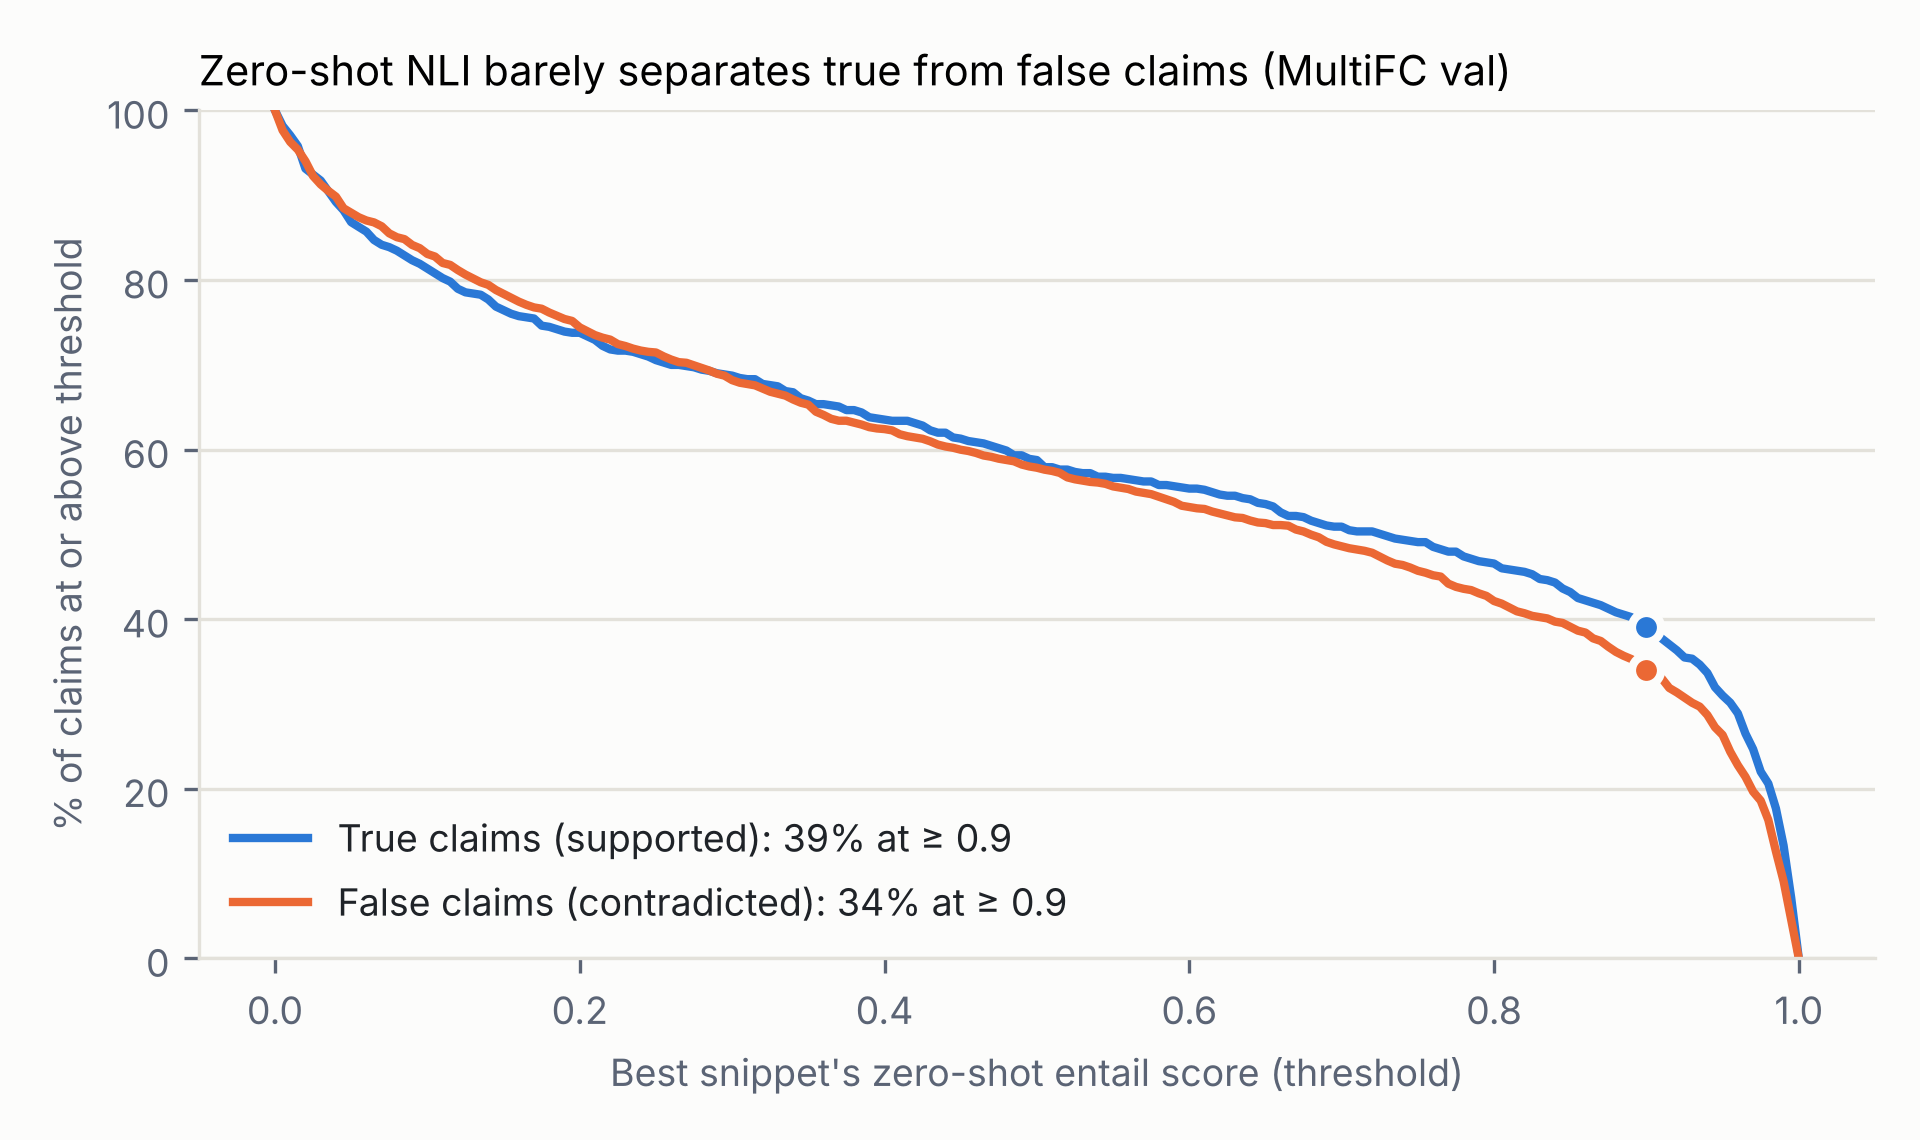
\includegraphics[width=0.78\textwidth]{figures/fig_entail_shortcut.png}
\caption{Share of true and false MultiFC validation claims whose best snippet reaches each zero-shot entailment score. The curves nearly overlap: snippets ``support'' false claims almost as often as true ones (\texttt{results/H5/zeroshot\_signal\_by\_label.json}).}
\label{fig:shortcut}
\end{figure}

\paragraph{Snippets often repeat the claim.}
Search results for a viral claim frequently restate it, whether it is true or false. A snippet with entailment of at least 0.9 exists for 39\% of true and 34\% of false claims (Figure~\ref{fig:shortcut}). ``The evidence agrees'' is therefore a weak signal, and ``supported'' is the hardest class for every evidence-based model. Youssef's error analysis found the same pattern in X-FACT Arabic, where 15 of 36 failures were false rumours repeated by the snippets.

\paragraph{Automatic labels teach shortcuts.}
The NLI v1 collapse is a concrete case of shortcut learning: labels copied from the claim's verdict taught the model to copy rather than compare. Small human-labelled gold sets were what exposed this, and they decided several model choices.

\paragraph{How far to trust the twin metrics.}
Three caveats temper the headline numbers. First, only 22.5\% of automatic \tw{B} twins are clean contradictions, so ESR mostly measures sensitivity to \emph{changed} evidence rather than to true contradictions. Second, the twin-trained head leans towards ``contradicted'': it labels 61\% of the supported source claims contradicted (40\% without the twin loss), so part of the ESR gain is bias. A paired ESR, counted only on sources not already called contradicted, still favours the twin loss (76.4\% vs 32.7\%, \texttt{results/Y5/diagnostics.csv}). Third, \tw{C} evidence has reranker relevance below 0.1 by construction, which makes the unrelated test relatively easy.

\paragraph{Arabic.}
About 85\% of Arabic errors are also errors on the English original, so most of the gap comes from the head rather than the language. Among the rest, translation is the main cause (12 of 20 analysed cases), and only 54\% of checked translations were fully correct. Entity features are English-only, which explains why removing them improves cross-lingual consistency.

\paragraph{Smaller can be better.}
The 4-bit Qwen3-4B matched or beat Qwen3-8B in every LLM role we tested. With limited compute, this argues for testing smaller models before scaling up.

\paragraph{Limitations.}
The \tw{B} generator needs claim-entity swaps and validation; the QLoRA models ran with one seed; the Arabic test sets are small and skewed; dialects are absent; the claim-extraction messages are template-based rather than real forwards; and MultiFC's evidence is often too weak to decide the claim.

% ---------------------------------------------------------------------
\section{Ethical Issues}
% ---------------------------------------------------------------------

\paragraph{Harm and over-reliance.}
A wrong ``false'' verdict can damage a person's reputation or public trust, and a confident wrong ``true'' can spread a rumour. TwinCheck is designed as an assistant, not an arbiter. It can answer ``unverified'', reports a calibrated confidence, and cites the snippets behind each verdict so that users can check them. The twin tests themselves are an ethical tool: they check whether the system's stated reason, the evidence, is the real one.

\paragraph{Bias and fairness.}
MultiFC is dominated by US fact-checking sites, the entity features work only in English, and no Arabic dialects are covered. We report every result per language, test a system without English-only features, and state the remaining gaps openly. Arabic users should not assume the same reliability as English users.

\paragraph{Privacy.}
Real forwarded messages can contain names, phone numbers and private details. We used no real messages: the claim-extraction set was built from public fact-checked claims, and every demo example is labelled ``illustrative''. All models run locally on our own GPUs, so no message is sent to a commercial API.

\paragraph{Data licences and consent.}
MultiFC is released for research use and AVeriTeC under CC BY-NC 4.0; we cite both and use them non-commercially. Human evaluation was carried out by team members only, with no outside participants.

\paragraph{Misuse.}
A fact-checker could be used to label opinions as ``false'' or to probe how to word claims that slip past checks. TwinCheck gives verdicts only from retrieved evidence, and the code is open so that the method can be examined.

\paragraph{Images.}
The verdict head never sees the AI-authenticity score from the vision module, so an AI-looking but genuine photo cannot by itself make a true post appear fake. Recent work found that adding deepfake-detector outputs to fact-checking pipelines can reduce accuracy \citep{sagar2026factorfake}, which supports this design rule.

\paragraph{Environmental cost.}
We used 4-bit models and small heads on free T4 GPUs, and kept the smaller Qwen3-4B wherever it performed as well as the 8B model.

% ---------------------------------------------------------------------
\section{Conclusion and Lessons Learned}
% ---------------------------------------------------------------------

We asked whether fact-checking verdicts follow the evidence. With one-change twins built from real claims, we found that on MultiFC the most accurate systems are those that read the evidence least (RQ1). A twin loss makes a small, interpretable verdict head follow the evidence: unrelated evidence is always recognised and swapped evidence is caught nine times in ten, for about one macro-F1 point (RQ2). Twins help a large language model as well: fine-tuned Qwen3-4B goes from recognising unrelated evidence 15\% of the time to 99\%. In Arabic, a fair system performs close to English and keeps three quarters of English verdicts, with translation quality as the main limit (RQ3).

\paragraph{Lessons learned.}
(1) Check the data before the model: leaked snippets and label noise shape every score. (2) Automatic labels teach shortcuts; small human-labelled gold sets keep evaluation honest. (3) Bigger is not always better: a 4-bit 4B model matched or beat the 8B model on free hardware. (4) Choose metrics that reward the right reason, not only the right answer. (5) State limits plainly: our \tw{B} twins are noisy, and ESR should always be read with its caveats.

\paragraph{Future work.}
Validated swaps of claim entities, human-labelled on-topic NLI pairs, multilingual entity matching, Arabic dialects, and real forwarded messages collected with consent.

% ---------------------------------------------------------------------
\section{Links: Code, Demo and Data}
% ---------------------------------------------------------------------
\begin{itemize}\setlength{\itemsep}{1pt}
  \item \textbf{Code repository:} \url{https://github.com/himaallu/Group-Project} (release tag \texttt{v1.0.1}). The script \texttt{run\_all.sh} reproduces the main tables, and \texttt{docs/implementation.md} lists every model, checkpoint and hyperparameter.
  \item \textbf{Demo:} Gradio app in \texttt{src/demo/app.py}, runnable in Colab via \url{notebooks/R10_demo_colab.ipynb}. \textcolor{red}{[Add the demo video link.]}
  \item \textbf{Fine-tuned reranker:} \url{https://huggingface.co/RathiAbeth/twincheck-reranker-v1}
  \item \textbf{Datasets:} MultiFC \citep{augenstein2019multifc} (authors' release; mirror \url{https://huggingface.co/datasets/pszemraj/multi_fc}); AVeriTeC \citep{schlichtkrull2023averitec}; X-FACT \url{https://github.com/utahnlp/x-fact}; M4FC \url{https://github.com/UKPLab/M4FC}. \textcolor{red}{[Add the AVeriTeC download link used by \texttt{src/data/load\_averitec.py}.]}
\end{itemize}

\section*{Team Contributions}
\textbf{Himasri} (integration, evaluation, report lead): repository, metrics, gold English NLI pairs, verdict head and twin loss, $\lambda$ grid and calibration, pipeline, ablations, bootstrap tests, Qwen3-4B comparisons. \textbf{Rathi} (code): English data and cleaning, reranker, English twins, NLI fine-tuning, explanations and offline index, demo, reproducibility. \textbf{Youssef} (Arabic and claims): X-FACT and M4FC data, Arabic NLI and gold pairs, claim extraction, Arabic twins and experiments. \textbf{Feba} (vision and baselines): baselines including the LLM judge, image side (reported in MAAI901). All four rated explanations and checked twins.

\bibliographystyle{plainnat}
\bibliography{refs}

\end{document}
